\documentclass[titlepage]{scrartcl}

%Referenzen zwischen unterschiedlichen Dateien
\usepackage{xr}
\externaldocument{theorie}

%Deutsche Sprachunterstützung
\usepackage[utf8]{inputenc}
\usepackage[ngerman]{babel}
\usepackage{marvosym}
\DeclareUnicodeCharacter{20AC}{\EUR}

%Für das Einbinden von Bildern
\usepackage{graphicx}

%Tabellen
\usepackage{array}

%Tabellen automatisch schoener
\usepackage{booktabs}

%Caption
\usepackage{caption}
\usepackage{subcaption}

%Formeln
\usepackage{mathtools}
\usepackage{amsmath}
\usepackage{amssymb}
\usepackage{amstext}
\usepackage{dsfont}

%\usepackage{mnsymbol}

%Vectorpfeile schöner
\usepackage{esvect}

%Formatierung
\usepackage[T1]{fontenc}
\usepackage{lmodern}
\usepackage{microtype}

%Schaltbilder malen
\usepackage[europeanresistors,cuteinductors,siunitx]{circuitikz}

%\usepackage[german=guillemets]{csquotes}

%Formatierungsanweisungen
\newcommand{\wichtig}[1]{\underline{\large{#1}}}
\newcommand{\aref}[1]{(s.Abb. \ref{#1})}
\newcommand{\R}{\mathbb{R}}
\newcommand{\K}{\mathbb{K}}
\newcommand{\C}{\mathbb{C}}

%\includeonly{theorie}
%\includeonly{theorie,versuchsdurchfuehrung,ergebnisse,anhang}
\begin{document}

\title{Geschwindigkeitsmessung mittels Pitotrohr}
\subtitle{PPG8}
\date{Januar 2014}
\author{Udo Beier \and Leon Brückner \and Valentin Olpp \and Marco Zech \and Sebastian Ziegler}
\maketitle
\tableofcontents
\newpage
\listoffigures
\listoftables
\newpage
\section{Vorwort}
Ursprünglich wurde das Michelson-Morley-Interferometer von Albert Abraham Michelson (1852 - 1931) und Edward William 
Morley (1838 - 1923) verwendet, um die Existenz eines Äthers, also eines möglicherweise existierenden Trägermediums von elektromagnetischen Wellen, 
zu überprüfen. Gäbe es einen solchen Äther, so müsste sich das Labor aufgrund der Erdrotation ebenfalls durch den Äther 
bewegen und zwar in wechselnder Richtung. Nach dem in der Theorie beschriebenen Aufbau würde dies eine Änderung des zu 
beobachtenden Interferenzmusters bewirken. Tatsächlich konnte unter korrekter Ausführung dieses Versuches allerdings 
niemals eine solche Verschiebung festgestellt werden, sodass die Idee des Äthers schließlich fallen gelassen werden 
musste. Dementsprechend bewegt sich das Licht unabhängig vom Bezugssystem des Beobachters immer mit der 
Lichtgeschwindigkeit c, was auch als Einsteinsches Relaltivitätsprinzip bekannt ist. Der Grund dafür ist schlicht, 
dass es die wesentliche Abänderung des Verständnisses von Raum und Zeit darstellt, welches schließlich zur 
Lorentz-Transformation und der speziellen Relativitätstheorie führte. Somit kommt diesem Experiment eine herausragende Rolle 
in der Entwicklung der modernen Physik zu. 

\section{Theorie}

\subsection{Kohärenzlänge und Kohärenzzeit}
Unter der Kohärenzlänge einer Lichtquelle versteht man die Länge, um die sich die durchlaufenen Wege zweier von der 
selben Lichtquelle stammenden Strahlen maximal unterscheiden dürfen, sodass noch eine räumlich und zeitlich konstante 
Interferenz zu beobachten ist. Das Phänomen, das diese Definition notwendig macht, ist, dass prinzipiell keine reale Lichtquellen eine über längere Zeit exakte 
Sinusschwingung mit konstanter Frequenz liefert, sondern sich mit der Zeit ein \enquote{Versatz} der Phase herausbildet. Es ist deswegen nicht 
mehr möglich, für eine Länge zwischen einem Maximum und einem weiteren Punkt auf dem Wellenzug, die zwar einem 
Vielfachen der Wellenlänge entspricht, aber auch die Kohärenzlänge überschreitet, wiederum auf ein Maximum zu schließen. \\
Die Kohärenzzeit bezeichnet die maximale Zeitdifferenz zwischen zwei Punkten auf dem Wellenzug, deren Abstand kleiner 
als die Kohärenzlänge ist, und ergibt sich deshalb im Vakuum zu 

\begin{equation}
t_{K} = \frac{l_{k}}{c},
\end{equation}

wobei hier $ t_{K} $ die Kohärenzzeit, $ l_{k} $ die Kohärenzlänge und c die Lichtgeschwindigkeit bezeichnet. \\
Bei Lasern ist die Kohärenzlänge meist verhältnismäßig groß und kann mehrere Kilometer erreichen, wohingegen bei anderen Lichtquellen, die etwa auf thermischer Emission beruhen, nur sehr kleine Kohärenzlängen erreicht werden. So liegt diese bei Glühbirnen im Bereich von Mikrometern. 

\subsection{Interferenz zweier Lichtstrahlen}
Werden zwei Lichtstrahlen, die in gleicher Richtung polarisiert sind, überlagert, so ergibt sich die tatsächliche Lichteinstrahlung durch Addition der beiden elektrischen Felder an diesem Ort. 
Seien $ \vec{E}_{1} $ und $ \vec{E}_{2} $ die elektrischen Felder des einfallenden Lichts mit: 
\begin{equation}
\vec{E}_{1} = \vec{e}_{p} \cdot E_{1} \cdot e^{i(\omega_{1}t - k_{1} \cdot r + \phi_{1})}
\end{equation} und 
\begin{equation}
\vec{E}_{2} = \vec{e}_{p} \cdot E_{2} \cdot e^{i(\omega_{2}t - k_{2} \cdot r + \phi_{2})}.
\end{equation}

Dabei sind $ E_{1}, E_{2} $ die Amplituden beider Felder, $ \omega_{1}, \omega_{2} $ die Frequenzen der beiden Schwingungen, $ r_{1}, r_{2} $ die zurückgelegten Wege der beiden Lichtstrahlen, $ k_{1}, k_{2} $ die Beträge der Wellenvektoren $ \vec{k_{1}}, \vec{k_{2}} $, die in Ausbreitungsrichtung zeigen sollen und $ \vec{e}_{p} $ der Einheitsvektor in Richtung der Polarisation. Weiter sind  $ \phi_{1} $ und $ \phi_{2} $ die Phasen des elektrischen Feldes bei $ r_{1}, r_{2}, t = 0 $. 
 
Als Summe über beide Felder ergibt sich zeitabhängig: 
\begin{equation}
\vec{E}_{1} + \vec{E}_{2} = \vec{e}_{p} \cdot (E_{1} \cdot e^{i(\omega_{1}t - k_{1} \cdot r_{1} + \phi_{1})} + E_{2} \cdot e^{i(\omega_{2}t - k_{2} \cdot r_{2} + \phi_{2})}).
\end{equation}

Mit $ \varphi_{1} = - k_{1} \cdot r_{1} + \phi_{1} $ und 
$ \varphi_{2} = - k_{2} \cdot r_{2} + \phi_{2} $ ergibt sich: 
\begin{equation}
\vec{E} = \vec{E}_{1} + \vec{E}_{2} = \vec{e}_{p} \cdot (E_{1} \cdot e^{i(\omega_{1}t + \varphi_{1})} + E_{2} \cdot e^{i(\omega_{2}t + \varphi_{2})}).
\end{equation}
Die Lichtintensität I ist nach \footnote{\cite[433f.]{feynman2011feynman}} proportional zum zeitlichen Mittel von $  \vec{E}_{reell} ^{2} $ über eine Schwingung, deshalb: 

\begin{equation}
\nonumber
\vec{E}_{reell}^{2} = 
(\vec{e}_{p} \cdot (E_{1} \cdot \cos(\omega_{1}t + \varphi_{1})) + E_{2} \cdot \cos(\omega_{2}t + \varphi_{2})))^{2} = 
(E_{1} \cdot \cos(\omega_{1}t + \varphi_{1}) + E_{2} \cdot \cos(\omega_{2}t + \varphi_{2}))^{2} = 
\end{equation}
\begin{equation}
E_{1}^{2} \cdot cos^{2}(\omega_{1}t + \varphi_{1}) + 2E_{1}E_{2} \cdot \cos(\omega_{1}t + \varphi_{1}) \cdot \cos(\omega_{2}t + \varphi_{2}) + E_{2}^{2} \cdot \cos^{2}(\omega_{2}t + \varphi_{2}).
\end{equation}


Die beiden quadratischen Terme können als Feldstärkequadrate der einzelnen Strahlen identifiziert werden, es bleibt der Mischterm: 
\begin{equation}
2E_{1}E_{2} \cdot \cos(\omega_{1}t + \varphi_{1}) \cdot \cos(\omega_{2}t + \varphi_{2}) = 
E_{1}E_{2} \cdot (\cos(t(\omega_{1} + \omega_{2}) + \varphi_{1} + \varphi_{2}) + \cos(t(\omega_{1} - \omega_{2}) + \varphi_{1} - \varphi_{2})).
\end{equation}
Für $ \omega_{1} = \omega_{2} $ (und damit auch $ k_{1} = k_{2} $) kann dies weiter vereinfacht werden zu: 
\begin{equation}
E_{1}E_{2} \cdot (\cos(2\omega t + \varphi_{1} + \varphi_{2}) + \cos(\varphi_{1} - \varphi_{2})),
\end{equation} für $ \omega_{1} \neq \omega_{2} $ würde sich im längerfristigen zeitlichen Mittel über dem Mischterm 0 ergeben, da beide Summanden zeitabhängig wären. 


Mittelt man nun über $  \vec{E}_{reell} ^{2} $, so folgt: 
\begin{equation}
\nonumber
<\vec{E}_{reell}^{2}> = 
\end{equation}
\begin{equation}
\nonumber
< E_{1}^{2} \cdot cos^{2}(\omega_{1}t + \varphi_{1}) + E_{2}^{2} \cdot \cos^{2}(\omega_{2}t + \varphi_{2}) + E_{1}E_{2} \cdot (\cos(2\omega t + \varphi_{1} + \varphi_{2}) + \cos(\varphi_{1} - \varphi_{2})) > = 
\end{equation}
\begin{equation}
\nonumber
\frac{E_{1}^{2}}{2} + \frac{E_{2}^{2}}{2} + E_{1}E_{2} \cdot \cos(\varphi_{1} - \varphi_{2}) = 
\end{equation}
\begin{equation}
\frac{E_{1}^{2}}{2} + \frac{E_{2}^{2}}{2} + E_{1}E_{2} \cdot \cos( k \cdot (r_{2} - r_{1}) + \phi_{1} - \phi_{2}).
\end{equation}

Bezeichnen $ I_{1}, I_{2} $ die Intensitäten der einfallenden Lichtstrahlen, so ergibt sich über $ I = \mu <\vec{E}_{reell}^{2}> $: 
\begin{equation}
\label{formel:intensitaet}
I = I_{1} + I_{2} + 2 \sqrt{I_{1} I_{2}} \cdot \cos( k \cdot (r_{2} - r_{1}) + \phi_{1} - \phi_{2}).
\end{equation}





\subsection{Das Michelson-Interferometer}

Das Michelson-Interferometer gehört zur Klasse der Zweistrahlinterferometer. Seine Funktionsweise beruht darauf, 
dass ein polarisierter Laserstrahl mit Hilfe eines halbdurchlässigen Spiegels aufgespalten wird (siehe dazu Abb.
\ref{pic:skizze_versuchsaufbau}). Beide Strahlen werden gespiegelt und so wieder am halbdurchlässigen Spiegel 
vereinigt. Aufgrund der unterschiedlich großen zurückgelegten Wegstrecken kommt es dort zu Interferenzeffekten,
die vom genauen Aufbau des Interferometers abhängen.\\
Verändert man die Länge von einem der beiden Wege, so ändert sich auch die Phasenverschiebung zwischen beiden 
Lichtstrahlen und nach (\ref{formel:intensitaet}) auch die Intensität der interferierenden Strahlen und ergibt eine verschobene 
Cosinus- oder gleichbedeutend Sinusfunktion abhängig von $ k $ mal der Laufwegsdifferenz. Durch Beobachtung der Verschiebung der Interferenzen kann also auf die Geschwindigkeit 
geschlossen werden, mit der sich die Länge des einen Weges ändert: 
Hat sich das Interferenzmuster genau um $ 2 \pi $ verschoben, so hat sich nach (\ref{formel:intensitaet}) $ k \cdot \Delta r $ um $ 2 \pi $ vergrößert oder verkleinert.
Ein $ \Delta N $ von 1 entspricht deswegen genau einer Längenänderung um $ \frac{\lambda}{2} $, also:


\begin{equation}
\Delta l = \frac{\lambda}{2} \cdot \Delta N. 
\label{form:ausdzumax_1}
\end{equation}


wobei $ \lambda $ die Wellenlänge des verwendeten Lasers ist und N die Anzahl der während der Längenänderung durchlaufenen Intensitätsmaxima ist. 
Durch zeitliches Ableiten ergibt sich:
\begin{equation}
\frac{dL}{dt} = \frac{\lambda}{2} \cdot \frac{dN}{dt}.
\label{form:ausdzumax}
\end{equation}


Weiterhin kann das vom Laser emittierte Strahlenbündel durch Einbringen von einer oder mehrerer Linsen zu einem 
divergenten Strahl oder einem breiteren, parallelen Strahlenbündel gewandelt werden. Durch eine solche Aufweitung kommt es 
zu weiteren Interferenzphänomenen, welche im nächsten Absatz detaillierter beschrieben werden. Oftmals geschieht dies mit 
Hilfe eines \enquote{Teleskops}, bei dem das Strahlenbündel eine Kombination aus konkaver und konvexer Linse 
durchläuft und danach parallel austritt. Im Falle eines zu Beginn ebenfalls parallelen Strahlenbündels, wie es 
vom Laser in guter Näherung emittiert wird, müssen dazu die beiden Brennpunkte aufeinander fallen.  \\

Die beobachtbaren Interferenzeffekte hängen maßgeblich von der genauen Ausrichtung der optischen Elemente im 
Strahlengang ab: 
Sind etwa die reflektierenden Spiegel nicht exakt senkrecht zum einfallenden Strahl ausgerichtet oder der 
halbdurchlässige Spiegel nicht in einem Winkel von exakt $ 45 ^\circ$  zum einfallenden Strahl justiert, so 
führt diese Verkippung der Spiegel zu deutlich sichtbaren Interferenzstreifen, da die Wellenfronten der beiden 
interferierenden Strahlen dann nicht parallel auf den Schirm treffen. (Abb.~\ref{verkippung}: Die Differenz 
zwischen den beiden gestrichelten Strecken entspricht dem Phasenversatz zwischen den beiden Wellen an dem 
entsprechenden Punkt auf dem Schirm. Der Versatz ändert sich in der Horizontalen.) Treffen sich weiter die 
beiden Strahlbündel bei Vereinigung auf dem halbdurchlässigen Spiegel nicht mittig am gleichen Punkt, so 
beobachtet man sehr deutlich Interferenzringe, da sich die Laufzeiten bei Verschieben des betrachteten 
Punkts unterschiedlich ändern. Beide Effekte verschieben sich bei einer Änderung der Laufzeitdifferenz um eine Wellenlänge
genau um ein Maximum und sind so für eine alternative \enquote{Zählung} der Interferenzmaxima geeignet. 

\begin{figure}
\centering
        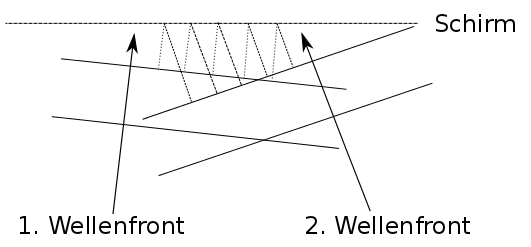
\includegraphics[width=.9\textwidth]{images/verkippung.png}
\caption{Darstellung der Interferenz zwischen zwei verkippten Wellenfronten}
\label{verkippung}
\end{figure}


\subsection{Thermische Längenänderung}
Wird ein Material erhitzt, so dehnt es sich in den meisten Fällen aus. Dies kann im Standard-Atom-Modell für einen Feststoff veranschaulicht werden: Wird dem Stoff thermische Energie zugeführt, bedeutet dies effektiv eine Zunahme der kinetischen Energie der Atomrümpfe. Dadurch nimmt die Amplitude von deren Schwingung um die Ruhelage zu und es kommt effektiv zu einer \enquote{Streckung} des Materials in alle Raumrichtungen. Eine exakte Beschreibung ist tatsächlich deutlich komplizierter und erfordert die Verwendung von Quantenmechanik. Im Allgemeinen ergibt sich kein einfacher Verlauf für $ l(T) $, allerdings kann die Längenänderung für einen bestimmten Temperaturbereich durch einen linearen Verlauf angenähert werden 

\begin{equation}
\frac{ \Delta l}{l_{0}} = \alpha(T) \cdot (T-T_{0}), 
\label{formel:ausdehnung}
\end{equation}

wobei $ l_{0} $ die eindimensionale Ausdehnung bei der Temperatur $ T_{0} $ ist. $ \alpha $ heißt der Längenausdehnungskoeffizient und ist insbesondere vom Material abhängig. 

\subsection{Überlegungen zu Wärmeleitung und Konvektion}
Für den Wärmestrom $ \vec{j} $ innerhalb eines Materials gilt: 

\begin{equation}
\vec{j} = - \kappa \cdot \nabla T, 
\label{form:j}
\end{equation}

wobei hier $ \kappa $ der Wärmeleitungskoeffizient ist sowie T die dreidimensionale Temperaturfunktion innerhalb des Materials. 

Weiter ergibt sich über
\begin{equation}
\int dt \int_{\partial V} -\vec{j} d \vec{f} = \int dt \int_{V} -\nabla \vec{j} dV = Q = m \cdot c \cdot \Delta T = \int_{V} \rho dV \cdot c \cdot \Delta T
\end{equation}
mit $c$ als massebezogene Wärmekapazität, $m$ als Masse, $\rho$ als Dichte. Durch Umschreiben in differenzielle Form folgt: 

\begin{equation}
\nabla \cdot \vec{j} = \rho \cdot c \cdot  \frac{\partial T}{\partial t}
\end{equation} 
und nach Einsetzen in \ref{form:j}: 

\begin{equation}
\frac{\partial T}{\partial t} = \frac{\kappa}{\rho \cdot c} \Delta T, 
\label{form:leitung}
\end{equation}
wobei hier $\Delta$ den Laplace-Operator darstellt. 
\\
Ein weiterer Effekt bei der Übertragung von Wärme ist die Konvektion. Diese bezeichnet allgemein den Transport von Wärme durch Strömungen in Flüssigkeiten oder Gasen. Die Konvektion lässt sich im Allgemeinen nur sehr schwer exakt beschreiben, da die Grundlage hierfür von der Navier-Stokes-Gleichung gebildet wird, die bis heute nicht allgemein gelöst wurde. Nach \cite{praktikumwaerme} gilt allerdings für den Wärmetransport von einem Gegenstand weg innerhalb eines Gases/ einer Flüssigkeit: 
\begin{equation}
\frac{dQ}{dt} \sim \Delta T,
\end{equation}
wobei $\Delta T$ die Differenz zwischen der Oberflächentemperatur des Gegenstandes und der Temperatur der Flüssigkeit/ des Gases ist. 
Nimmt man an, dass der Wärmeleitungskoeffizient innerhalb des Gegenstandes relativ hoch ist, was im Falle von Metall durchaus gerechtfertigt ist, so kann dessen Temperatur als konstant innerhalb des Gegenstandes angenommen werden. 
Im hier durchgeführten Experiment soll die Erwärmung eines Metallstabes von etwa $ -130 ^{\circ} C $ auf Raumtemperatur untersucht werden. Somit ergibt sich: 

\begin{equation}
\frac{dQ}{dt} \sim  \frac{dT_M}{dt} \sim (T_{M} - T_{R}). 
\label{form:konvektion1}
\end{equation}

Als Lösung einer derartigen Differentialgleichung ergibt sich eine e-Funktion 
\begin{equation}
k \cdot e^{a \cdot t} + b
\label{form:konvektion2}
\end{equation}
, auf die Bestimmung der Konstanten $k$ und $a$ und $b$ soll hier nicht weiter eingegangen werden. 

\subsection{Leidenfrost-Effekt}
Der Leidenfrost-Effekt beschreibt ursprünglich das Verhalten von Wassertropfen auf heißen Herdplatten. Wird ein Wassertropfen auf eine heiße Platte gegeben, verdampft die untere Oberfläche des Tropfens sehr schnell und bildet eine Schicht aus Wasserdampf, die den restlichen Tropfen vor weiterer Wärmeübertragung isoliert. Dadurch kann der Tropfen für längere Zeit auf der heißen Herdplatte gleiten, ohne zu verdampfen.
Ein ähnlicher Effekt entsteht, wenn Metall in flüssigen Stickstoff getaucht wird. Der Stickstoff rund um das Metall verdampft sehr schnell und bildet eine isolierende Schicht, was das Abkühlen des Metalls erschwert.

\section{Versuchsdurchführung}
\subsection{Herstellung des Rohres}
Für diesen Versuch wurde in einem CAD-Programm das Modell eines Pitotrohres (s. Abb. \ref{skizze-ks} für eine Skizze und Abb. \ref{render-ks} für ein 3D-Rendering) erstellt und dieses in einem 3D-Drucker gedruckt. Nach einigen Versuchen haben wir es so geschafft, ein funktionsfähiges Pitot-Rohr herzustellen.
\begin{figure}
\centering
	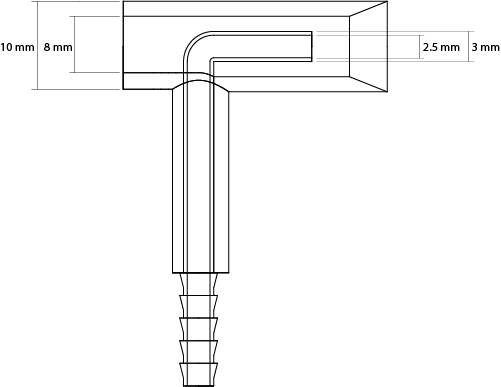
\includegraphics[width=.8\textwidth]{images/ks-zeichnung.png}
	\caption{Skizze des Messsondenmodels}
	\label{skizze-ks}
\end{figure}
\begin{figure}
\centering
	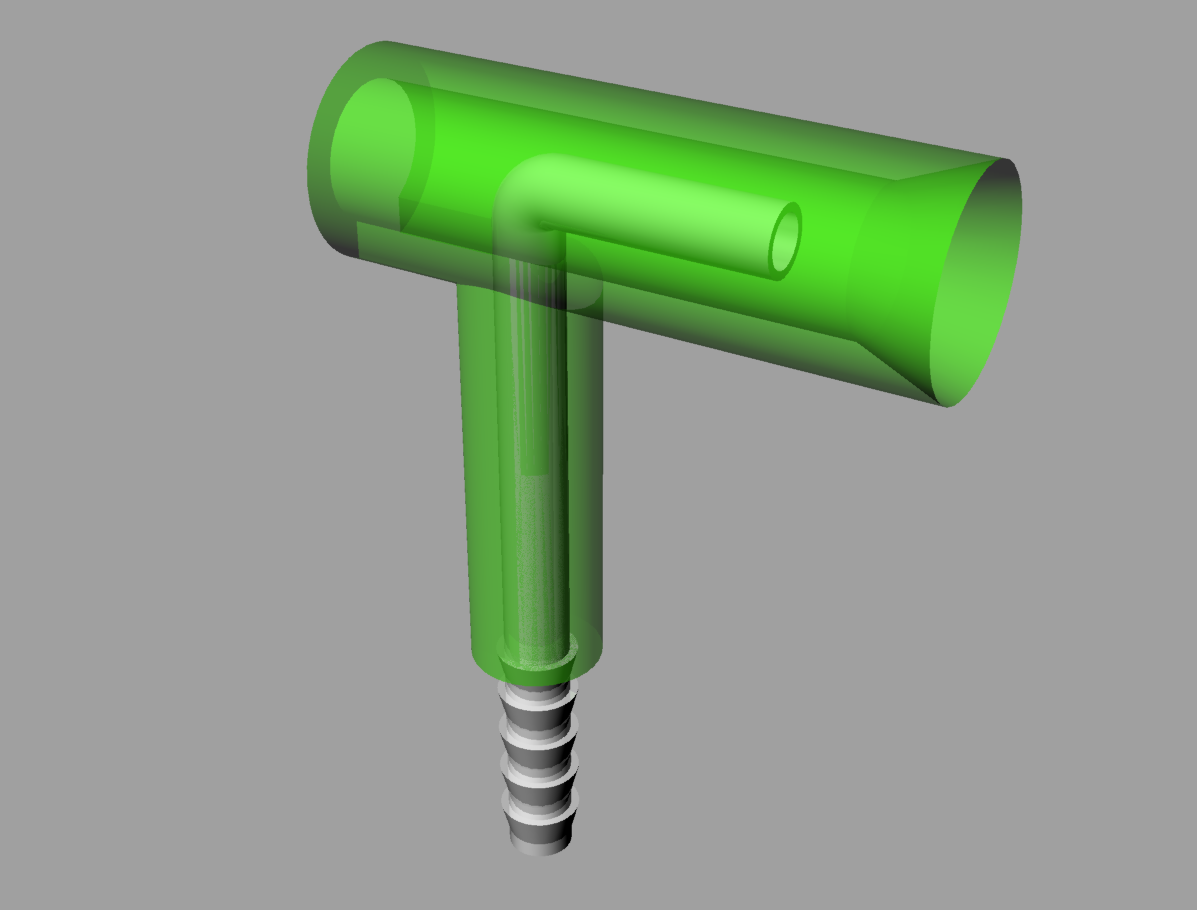
\includegraphics[width=.8\textwidth]{images/ks-render.png}
	\caption{3D-Rendering des Messsondenmodels}
	\label{render-ks}
\end{figure}
\subsection{Messung der Fahrgeschwindigkeiten}
Um die Geschwindigkeiten des fahrenden Autos zu messen, wurde das Pitotrohr am Dach des Autos befestigt (Siehe Abbildung \ref{rohre}), zusammen mit einer schon vorrätigen Prandtlsonde, welche zur Messung des statischen Druckes verwendet wurde. Diese sind mit einem Feinmanometer im Inneren des Autos verbunden worden. Mit einer ersten Kamera wurde der Stand des Manometers sowie parallel die von einem GPS-Sensor ausgegebene Geschwindigkeit aufgenommen (Siehe Abbildung \ref{messung}), mit einer zweiten die Anzeige des Tachometers. Die beiden Aufnahmen wurden über die Audiospur synchronisiert, um die drei Geschwindigkeiten zu jeweils einem bestimmten Zeitpunkt auswerten zu können.

\begin{figure}
\centering
	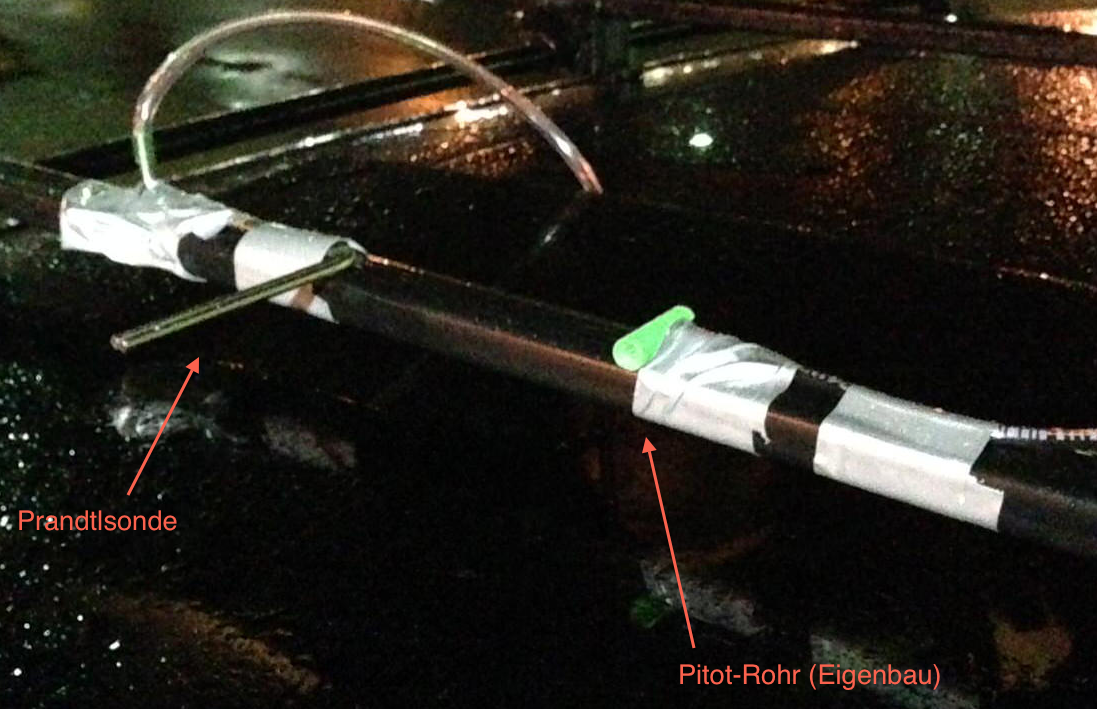
\includegraphics[width=.8\textwidth]{images/rohre-kommentiert.png}
	\caption{Bild des Versuchsaufbaus auf dem Autodach}
	\label{rohre}
\end{figure}

\begin{figure}
\centering
	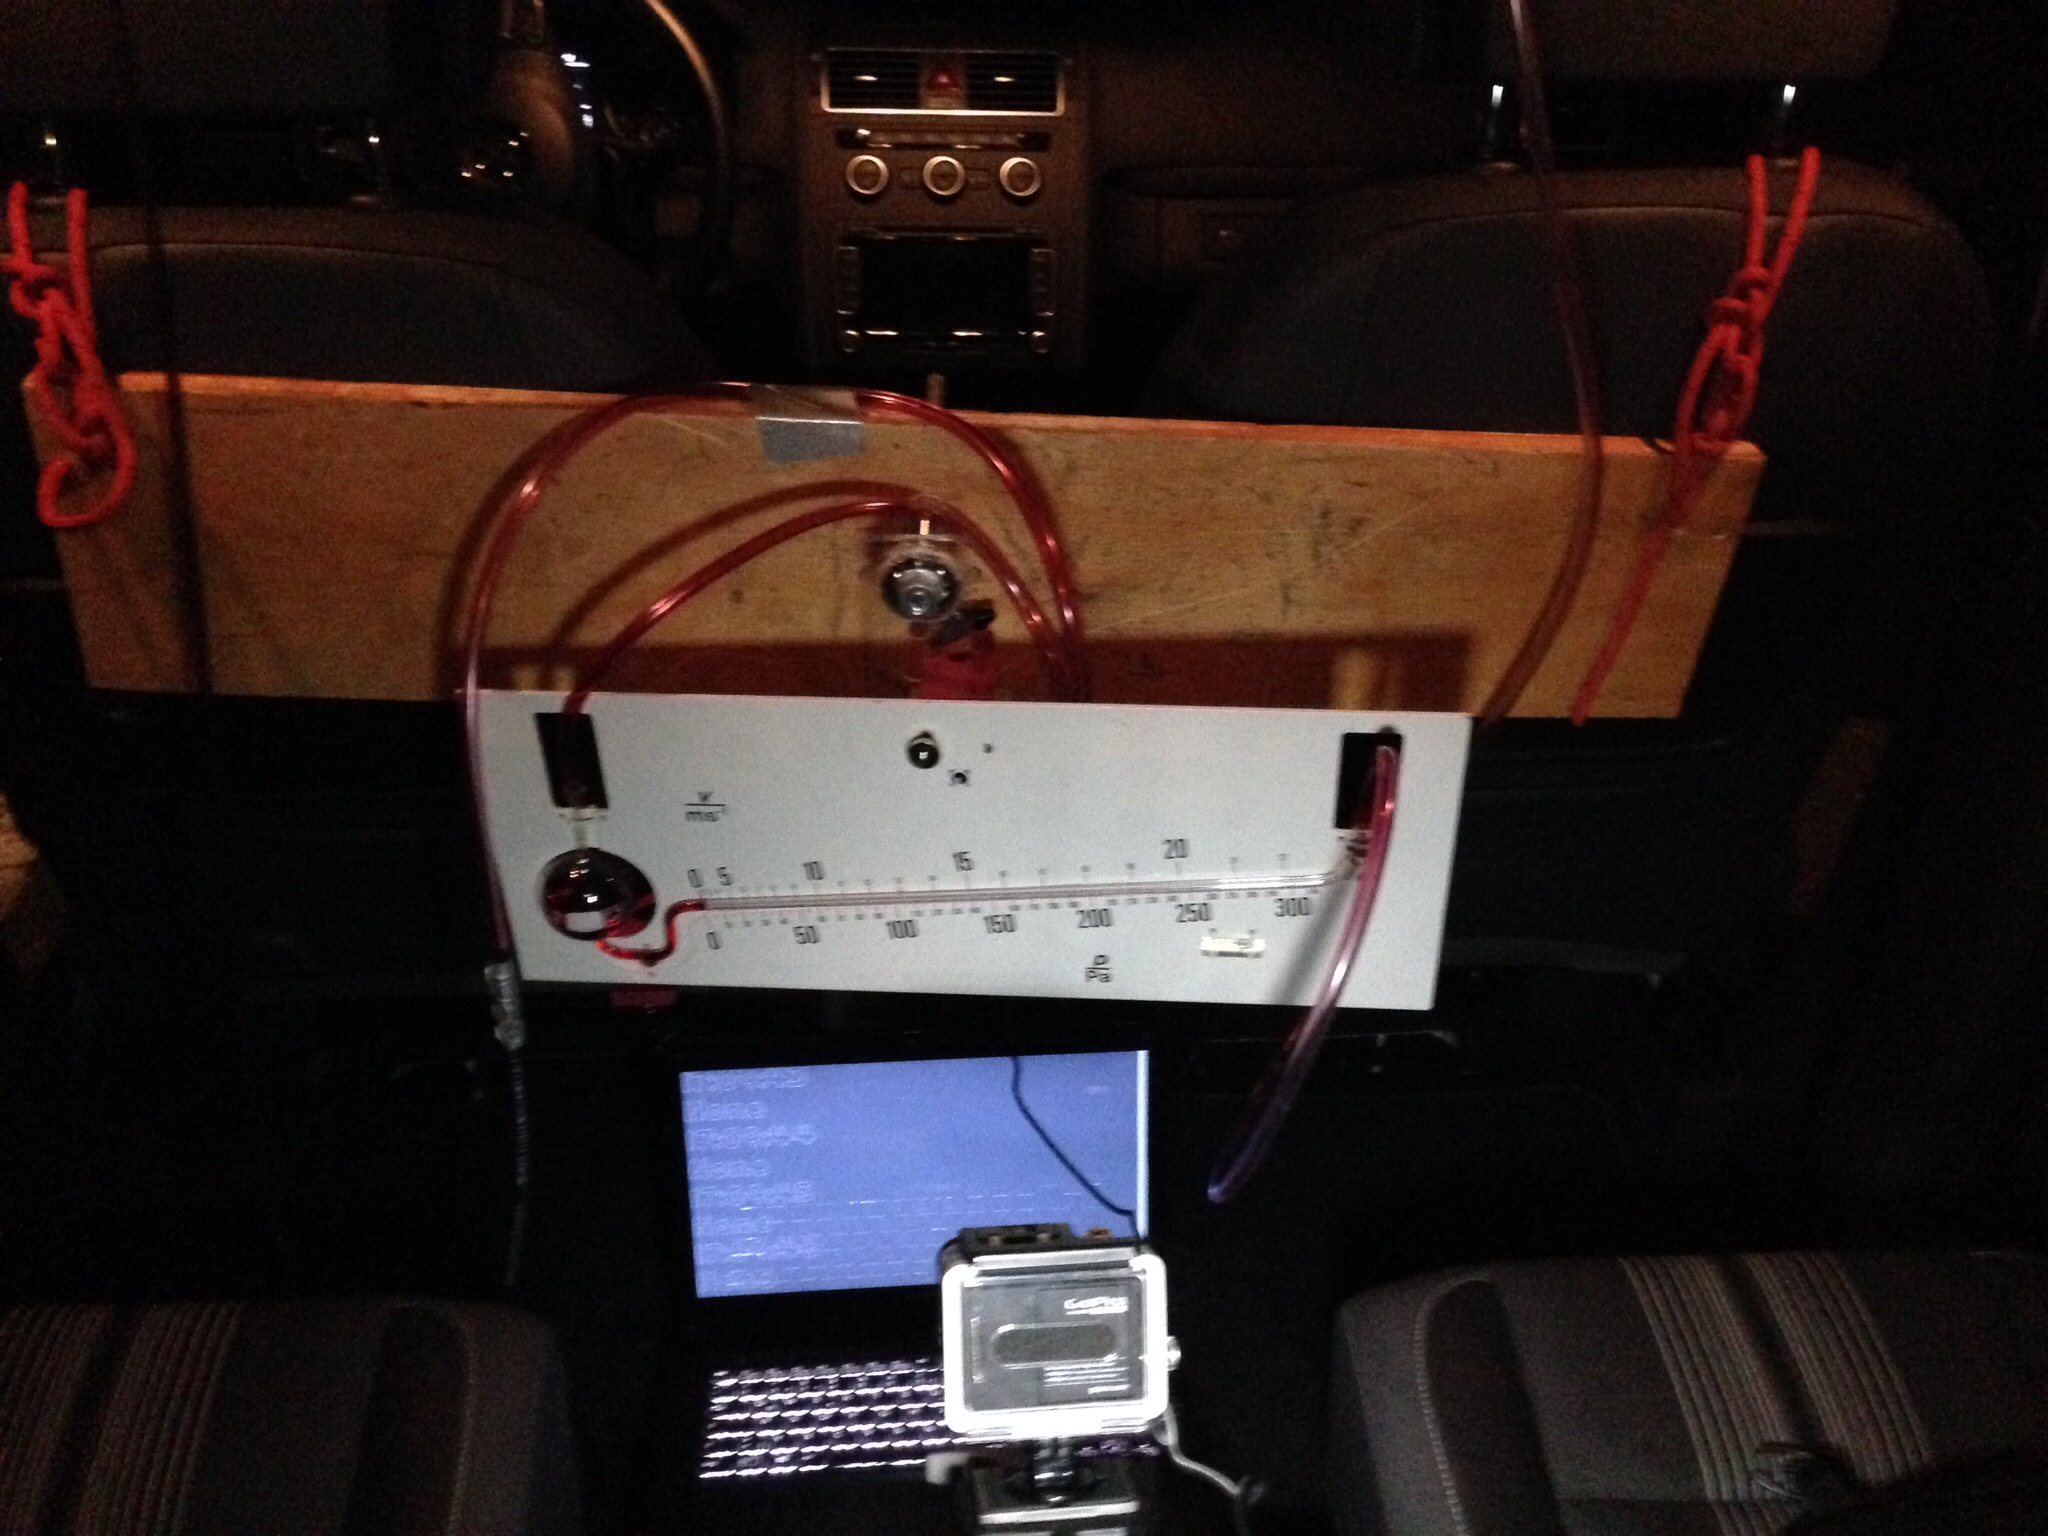
\includegraphics[width=.8\textwidth]{images/messung.jpg}
	\caption{Feinmanometer und Laptop mit GPS-Sensor}
	\label{messung}
\end{figure}

\subsection{Aufhängung des Feinmanometers}
Um mit dem Feinmanometer messen zu können, muss es genau senkrecht zur Beschleunigung ausgerichtet werden. Dies wurde im Auto mittels einer kardanischen Aufhängung realisiert (Siehe Abbildung \ref{aufhängung}): in eine frei im Auto, parallel zur Windschutzscheibe hängende Holzplatte wurde das Manometer mittels eines Kugellagers an einer Gewindestange befestigt und diese in ein Loch in der Mitte der Holzplatte eingelassen. Dies garantiert die waagrechte Ausrichtung des Manometers im Auto und gleicht leichtere Erschütterungen aus. 


\begin{figure}
\centering
	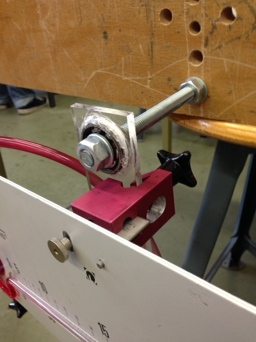
\includegraphics[width=.5\textwidth]{images/aufhaengung.JPG}
	\caption{Aufhänung des Feinmanometers}
	\label{aufhängung}
\end{figure}

\section{Darstellung der Ergebnisse und Auswertung}

\subsection{Darstellung der Ergebnisse}
Mit der oben beschriebenen Messmethode, wurden folgende Werte gemessen:
\begin{table}

\begin{tabular}{|c|c|}
\hline 
t in s & dN/dt in 1/10s \\ 
\hline
20	&34\\ 
\hline
40	&29\\ 
\hline
60	&32\\ 
\hline
80	&28\\ 
\hline
100	&31\\ 
\hline
120	&25\\ 
\hline
140	&28\\ 
\hline
160	&24\\ 
\hline
180	&27\\ 
\hline
200	&24\\ 
\hline
220	&32\\ 
\hline
240	&25\\ 
\hline
260	&24\\ 
\hline
280	&27\\ 
\hline	
300	&26\\ 
\hline
320	&25\\ 
\hline
340	&27\\ 
\hline
420	&29\\ 
\hline	
440	&29\\ 
\hline
460	&26\\ 
\hline
480	&25\\ 
\hline
500	&26\\ 
\hline
560	&26\\ 
\hline
580	&22\\ 
\hline	
600	&25\\ 
\hline
620	&22\\ 
\hline
640	&21\\ 
\hline
660	&20\\ 
\hline
680	&23\\ 
\hline
700	&21\\ 
\hline
760	&22\\ 
\hline
780	&20\\ 
\hline
800	&24\\ 
\hline
820	&22\\ 
\hline
840	&24\\ 
\hline
860	&23\\ 
\hline
880	&22\\ 
\hline
900	&20\\ 
\hline
920	&22\\ 
\hline
940	&20\\ 
\hline
960	&21\\ 
\hline
980	&22\\ 
\hline
1000&	18\\ 
\hline
1080&	19\\ 
\hline	
1100&	19\\ 
\hline
1120&	18\\ 
\hline
1160&	17\\ 
\hline
1180&	16\\ 
\hline
1200&	18\\ 
\hline
1220&	18\\ 
\hline
1240&	16	\\ 
\hline
1260&	17\\ 
\hline
1280&	15\\ 
\hline
1300&	18\\ 
\hline
1320&	16\\ 
\hline
1340&	15\\ 
\hline
1360&	14\\ 
\hline
1440&	13\\ 
\hline
1460&	12\\ 
\hline
1480&	12	\\ 
\hline
1500&	13\\ 
\hline
1520&	12\\ 
\hline
1540&	12\\ 
\hline
1560&	10	\\ 
\hline
1580&	12\\ 
\hline
1600&	12\\ 
\hline
1640&	9\\ 
\hline
1660&	8\\ 
\hline
1680&	8\\ 
\hline
1700&	8\\ 
\hline
1720&	9\\ 
\hline
1740&	8\\ 
\hline
1760&	8\\ 
\hline
1780&	8\\ 
\hline
1840&	7\\ 
\hline
1860&	6\\ 
\hline
1880&	7\\ 
\hline
1900&	6\\ 
\hline
1920&	6\\ 
\hline
1940&	6\\ 
\hline
2000&	5\\ 
\hline
2020&	5\\ 
\hline
2040&	5\\ 
\hline
2060&	5\\ 
\hline
2080&	5\\ 
\hline
2160&	5\\ 
\hline
2180&	4\\ 
\hline
2200&	4\\ 
\hline
2220&	3\\ 
\hline
\end{tabular} 

\label{tbl_1}
\caption{Anzahl der innerhalb von 10s durchgelaufenen Ringe in Abhängigkeit der Zeit}
\end{table}

\begin{comment}

\begin{figure}
        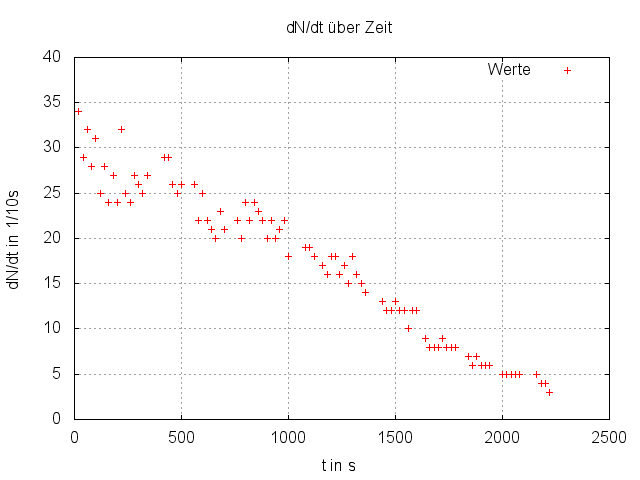
\includegraphics[width=.9\textwidth]{images/dNdt(t).png}
\caption{Anzahl der innerhalb von 10s druchgelaufenen Ringe in Abhängigkeit der Zeit}
\label{dNdt(t)}
\end{figure}


\end{comment}

Beim Betrachten von \ref{dNdt(t)} fällt sofort auf, dass die Messwerte bei großen Werten von dN/dt wesentlich mehr streuen, was darauf zurückzuführen ist, dass das Zählen der Ringe bei größeren Werten von dN/dt mehr Schwierigkeiten bereitet hat.
Eine Tabelle der Temperatur des Stabes in Abhängigkeit der Zeit ist im Anhang zu finden. \\
\ref{T(t)}

\begin{comment}

\begin{figure}
	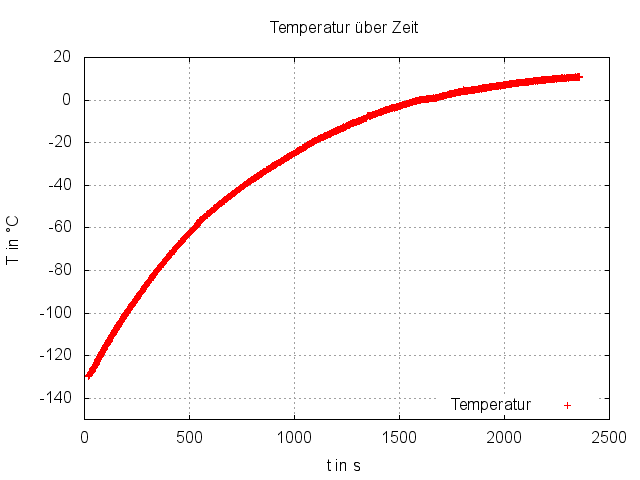
\includegraphics[width=.9\textwidth]{images/T(t).png}
\label{T(t)}
\caption{Temperatur in Abhängigkeit der Zeit}
\end{figure}

\end{comment}

An der Temperaturkurve ist bei $ 0 ^{\circ} C $ ein kurzes Gleichbleiben der Temperatur zu beobachten. Dies ist darauf zurückzuführen, dass sich Eis um den Stab gebildet hat. Dieses schmilzt bei $ 0 ^{\circ} C $ und hält den Stab so kurzzeitig auf einer konstanten Temperatur.

\subsection{Auswertung}
Aus den gemessenen Daten kann der Wärmeausdehnungskoeffizient $ \alpha $ des verwendeten Stabes in Abhängigkeit von der Temperatur bestimmt werden. Dafür werden in dieser Auswertung zwei verschiedene Methoden verwendet und anschließend miteinander verglichen.

\subsubsection{Einteilung der Messwerte in Fraktionen}
Bei dieser Methode werden die Messwerte möglichst gleichmäßig in Fraktionen eingeteilt und jeweils innerhalb dieser der Mittelwert von dN/dt gebildet.\\(Die Mittelwertbildung ist aus mehreren Gründen gerechtfertigt: Zum Einen wird gerade ein gemittelter Wärmeausdehnungskoeffizient bestimmt. Zum anderen kann dN/dt in den Fraktionen als linear approximiert werden, wodurch sich Abweichungen vom Mittelwert durch die Linearität gegenseitig aufheben.) Außerdem werden aus den zu den Fraktionen passenden Zeitintervallen die entsprechenden Zeitdifferenzen errechnet. Aus den so bestimmten Größen kann dann für jede Fraktion ein mittlerer Wärmeausdehnungskoeffizient folgendermaßen ermittelt werden:

\begin{equation}
\alpha(T)=\frac{\Delta L(T)}{L_{0}} \cdot \Delta T
\end{equation}

Aus $ \Delta L = \frac{\lambda}{2} \cdot \Delta N $ folgt:

\begin{equation}
\alpha (T)= \frac{\lambda}{2} \cdot \frac{\Delta N(T)}{L_0} \cdot \Delta T
\end{equation}

\begin{table}
\begin{tabular}{|c|c|c|}
\hline
Fraktion&	Zeitintervalle in s	& $\Delta T $ in $ ^{\circ} C$ \\
\hline
1		&[20, 180]		&26,5\\
\hline
2		&[200, 340]		&18,9\\
\hline
3		&[420, 500]		&8,7\\
\hline
4		&[560, 700]		&11,1\\
\hline
5		&[760, 880]		&7,9\\
\hline
6		&[900,1000]		&6,1\\
\hline
7		&[1080,1120]		&1,9\\
\hline
8		&[1160,1260]		&4,4\\
\hline
9		&[1280,1360]		&3,6\\
\hline
10		&[1440,1600]		&4,6\\
\hline
11		&[1640,1780]		&2,9\\
\hline
12		&[1840,1940]		&1,8\\
\hline
13		&[2000,2080]		&1,3\\
\hline
14		&[2160,2220]		&0,7\\
\hline
\end{tabular}

\caption{Einteilung in Fraktionen}
\label{tbl_2}
\end{table}



Innerhalb dieser Fraktionen ergeben sich folgende Mittelwerte mit zugehörigen Fehlern:

\begin{table}
\begin{tabular}{|c|c|c|}

\hline
Fraktion	&Mittelwert von dN/dt in 1/10s	&Fehler von dN/dt in 1/10s \\
\hline
1		&28,67				&1,08\\
\hline
2		&26,25				&0,92\\
\hline
3		&27					&0,84\\
\hline
4		&22,5				&0,73\\
\hline
5		&22,43				&0,53\\
\hline
6		&20,5				&0,62\\
\hline
7		&18,67				&0,33\\
\hline
8		&17					&0,37\\
\hline
9		&15,6				&0,68\\
\hline
10		&12					&0,29\\
\hline
11		&8,25				&0,16\\
\hline
12		&6,33				&0,21\\
\hline
13		&5					&0\\
\hline
14		&4					&0,41\\
\hline
\end{tabular}
\caption{Mittelwerte und Fehler von dN/dt}
\label{tbl_3}
\end{table}


An Tabelle \ref{tbl_3} fällt sofort auf, dass der Fehler in Fraktion 13 Null ist. Dies resultiert daraus, dass alle in dieser Fraktion zusammengefassten Werte gleich 5/10s sind.


\begin{comment}

\begin{figure}
        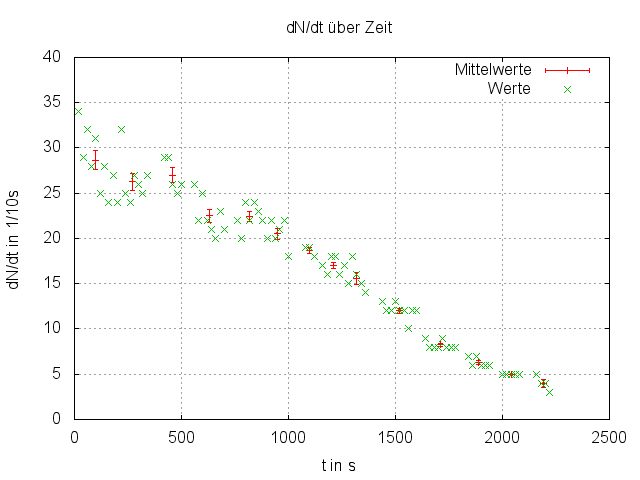
\includegraphics[width=.9\textwidth]{images/dNdt(t)MWmitaltenWerten.png}
\caption{Einteilung in Fraktionen}
\label{dNdt(t)MWmitaltenWerten}
\end{figure}

\end{comment}

\ref{dNdt(t)MWmitaltenWerten}

Für die Fehlerabschätzung von $ \alpha $ wird eine Fehlerfortpflanzung durchgeführt.
Dabei sind die Fehler von $ \lambda $  und  $ \Delta T $ vernachlässigbar klein. Im Fall von $ \Delta T $ ist der Fehler sogar nicht ermittelbar, da auf Grund der Benutzung von CASSY diesbezüglich keine ausreichenden Angaben vorhanden sind.

Der Fehler von $ L_{0} $ ist laut Versuchsaufbau $ 1 mm $.

Die Fehlerfortpflanzung liefert:

\begin{equation}
\Delta (\alpha) = \frac{\lambda}{2 \cdot \Delta T} \cdot \sqrt{\frac{1}{L_{0}^{2}} \cdot (\Delta(\Delta N))^{2} + \frac{(\Delta N)^{2}}{(L_{0})^{4}} \cdot (\Delta L_{0})^{2}}
\end{equation}


Es ergibt sich so:

\begin{table}
\begin{tabular}{|c|c|c|}
\hline
Mittlere Temperatur in $^{\circ}C$ &$ \alpha $ in $ 10^{-5}\frac {1}{^{\circ}C} $	&Fehler von $ \alpha $ in $ 10^{-5} \frac{1}{^{\circ}C}  $ \\
\hline
-115,6&				1,896	&		0,072\\
\hline
-90,2	&			2,129	&		0,075\\
\hline
-66,9	&			2,719	&		0,085\\
\hline
-50,1	&			3,108	&		0,101\\
\hline
-35,9	&			3,731	&		0,089\\
\hline
-27,9	&			3,680	&		0,112\\
\hline
-19,2	&			4,305	&		0,078\\
\hline
-14,0	&			4,231	&		0,093\\
\hline
-9,3	&			3,797	&		0,166\\
\hline
-2,1	&			4,571	&		0,112\\
\hline
2,1		&		4,362		&	0,086\\
\hline
5,3		&		3,851		&	0,128\\
\hline
7,7		&		3,370		&	0,011\\
\hline
9,4		&		3,755		&	0,385\\
\hline
\end{tabular}
\label{tbl_4}
\caption{Wärmeausdehnungskoeffizient in Abhängigkeit der Temperatur}
\end{table}

\begin{comment}

\begin{figure}
        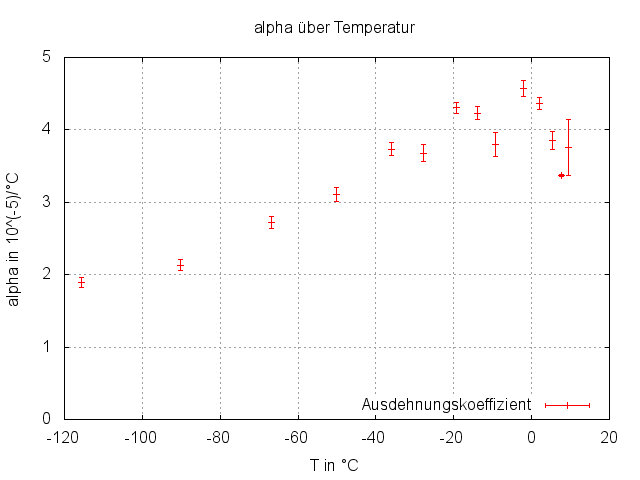
\includegraphics[width=.9\textwidth]{images/alpha(T).png}
\caption{Wärmeausdehnungskoeffizient in Abhängigkeit der Temperatur}
\label{alpha(T)}
\end{figure}

\end{comment}


\subsubsection{Berechnung des Ausdehnungskoeffizienten durch approximatives Fitten}

Bei dieser Methode werden dN/dt und T(t) gefittet und daraus der Ausdehnungskoeffizient in Abhängigkeit der Temperatur bestimmt.

dN/dt lässt sich gut mit einem Polynom 5. Grades approximieren:

\begin{equation}
 N^{*} := dN/dt 
\end{equation}

Dabei ergibt sich für 


\begin{equation}
N^{*}(t)=a_{0}+a_{1} \cdot t+a_{2}t^{2}+a_{3}t^{3}+a_{4}t^{4}+a_{5}t^{5} :
\end{equation}

$
 a_{0} =(3,153 \pm 0,104) s^{-1} 
$

$
a_{1}=(-0,00311 \pm 0,00097)s^{-2}
$

$
a_{2}=(5,78 \pm 2,65)10^{-6}s^{-3}
$

$
a_{3}=(-5,83 \pm 2,99)10^{-9}s^{-4}
$

$
a_{4}=(2,33 \pm 1,47)10^{-12}s^{-5}
$

$
a_{5}=(-3,21 \pm 2,62)10^{-16}s^{-6} 
$\\


\begin{comment}

\begin{figure}
        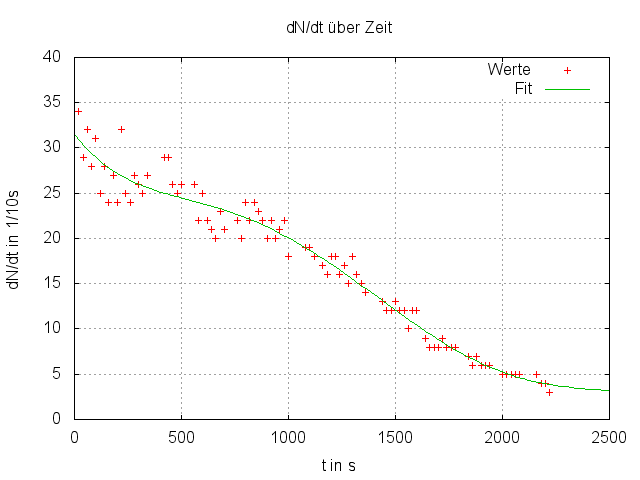
\includegraphics[width=.9\textwidth]{images/Fit dNdt(t).png}
\caption{Fit von dN/dt}
\label{Fit dNdt(t)}
\end{figure}

\end{comment}

T(t) lässt sich sehr gut mit einer e-Funktion approximieren:

Dabei ergibt sich für $ T(t) = a \cdot e^{bt} + c $ :

$a = (-154,01 \pm 0,04)^{\circ}C$,
$b=(-0,0012499 \pm 0,0000011)s^{-1}$,
$c=(19,91 \pm 0,042)^{\circ}C$

\begin{comment}

\begin{figure}
        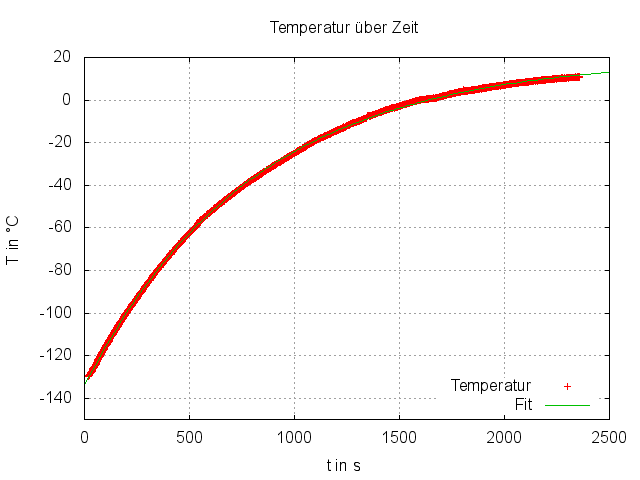
\includegraphics[width=.9\textwidth]{images/Fit T(t).png}
\caption{Fit von T(t)}
\label{Fit T(t)}
\end{figure}

\end{comment}

Herleitung einer Formel zur Berechnung des Ausdehnungskoeffizienten:

Wegen $ \Delta L = \alpha \cdot L_{0} \cdot \Delta T $ folgt: 
\\
\begin{equation}
\alpha (T) = \frac{1}{L_{0}} \frac{\partial L}{\partial T}
\end{equation}
Außerdem gilt: 
\begin{equation}
L = \frac{\lambda}{2} N
\end{equation}

\begin{equation}
\Rightarrow \alpha(T) = \frac{1}{L_{0}} \frac{\lambda}{2} \frac{\partial N}{\partial T} = \frac{\lambda}{2} \cdot L_{0} \frac{\partial N}{\partial t} \frac{\partial t}{\partial T}
\end{equation}

\begin{equation}
\Rightarrow \alpha (T) = \frac{\lambda}{2 \cdot L_{0}} \frac{N^{\cdot}(t(T))}{T^{\cdot}(t(T))}
\end{equation} 
mit 

Dann ergibt sich folgender Graph:

\begin{comment}

\begin{figure}
        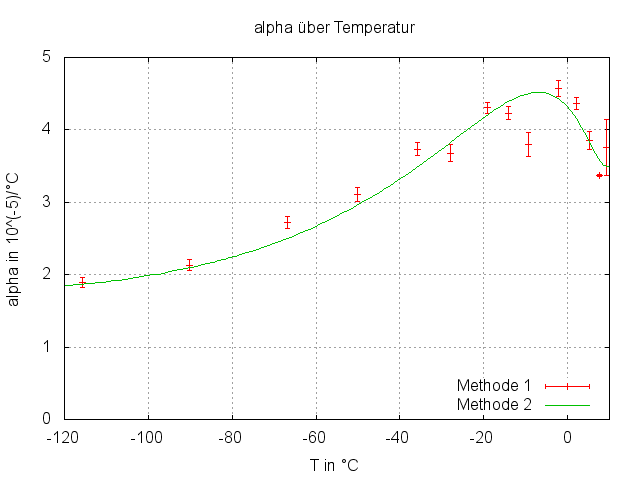
\includegraphics[width=.9\textwidth]{images/alpha(T)mitFit.png}
\caption{Vergleich zwischen Methode 1 und 2}
\label{alpha(T)mitFit}
\end{figure}

\end{comment}

\bibliographystyle{natdin}
\pagebreak
\begin{thebibliography}{9}
\bibitem[Demt]{roeder} DEMTRÖDER, Wolfgang. Experimentalphysik 1: Mechanik und Warme. Springer DE, 2005.
\bibitem[Reib]{wiki} Wikipedia. Tabellarische Auflistung von Rollreibungskoeffizienten. http://de.wikipedia.org/wiki/Rollreibung. (11. Januar 2014)
\bibitem[Eul]{eul} Wikipedia. Tabellarische Auflistung von Rollreibungskoeffizienten. http://de.wikipedia.org/wiki/Rollreibung. (11. Januar 2014)
\end{thebibliography}

\newpage
%\bibliographystyle{natdin}
%\bibliography{literature}
\section{Anhang}
%\subsection{Winkelabhängigkeit}
% Table generated by Excel2LaTeX from sheet 'Tabelle1'
\begin{table}[htbp]
  \centering
  \caption{Winkelabhängigkeit des Pitotrohrs}
    \begin{tabular}{rrrrrrrr}
    \toprule
    v=4,3 m/s &       &       & v=10,3 m/s &       &       & v=14,2 m/s &  \\
    \midrule
    Druck in Pa & Winkel in Grad &       & Druck in Pa & Winkel in Grad &       & Druck in Pa & Winkel in Grad \\
    18    & 0     &       & 58    & 0     &       & 113   & 0 \\
    19    & 7     &       & 57    & 7     &       & 111   & 7 \\
    18    & 15    &       & 57    & 15    &       & 113   & 15 \\
    18    & 23    &       & 55    & 23    &       & 111   & 23 \\
    19    & 31    &       & 53    & 31    &       & 111   & 31 \\
    16    & 39    &       & 51    & 39    &       & 106   & 39 \\
    16    & 47    &       & 42    & 47    &       & 84    & 47 \\
    14    & 56    &       & 38    & 56    &       & 70    & 56 \\
    7     & 64    &       & 20    & 64    &       & 57    & 64 \\
    \bottomrule
    \end{tabular}%
  \label{tab:Winkel}%
\end{table}%

% Table generated by Excel2LaTeX from sheet 'Tabelle1'
\begin{table}[htbp]
  \centering
  \caption{Winkelabhängigkeit der Prandtlsonde}
    \begin{tabular}{rr}
    \toprule
    v=10,3 m/s &  \\
    \midrule
    Druck in Pa & Winkel in Grad \\
    63    & 0 \\
    64    & 10 \\
    63    & 20 \\
    61    & 30 \\
    59    & 40 \\
    55    & 50 \\
    45    & 60 \\
    36    & 70 \\
    \bottomrule
    \end{tabular}%
  \label{tab:Winkelnormalrohr}%
\end{table}%

%\subsection{Kalibration}
% Table generated by Excel2LaTeX from sheet 'Tabelle1'
\begin{table}[htbp]
  \centering
  \caption{Kalibration Teil 1}
    \begin{tabular}{rr}
    \toprule
    Geschwindigkeit Windmesser in m/s & Druck Pitotrohr in Pa \\
    \midrule
    4,6   & 11 \\
    6,2   & 20 \\
    7,4   & 30 \\
    9     & 45 \\
    11,1  & 70 \\
    13,1  & 97 \\
    14    & 111 \\
    16,1  & 152 \\
    \bottomrule
    \end{tabular}%
  \label{tab:Kalibration1}%
\end{table}%
% Table generated by Excel2LaTeX from sheet 'Tabelle1'
\begin{table}[htbp]
  \centering
  \caption{Kalibration Teil 2}
    \begin{tabular}{rrrr}
    \toprule
    Geschwindigkeit Pitotrohr in m/s & Fehler & Abweichung &  \\
    \midrule
    4,2   & 0,38 & 0,4   &  \\
    5,7   & 0,28 & 0,5   &  \\
    7     & 0,23 & 0,4   &  \\
    8,5   & 0,19 & 0,5   &  \\
    10,6  & 0,15 & 0,5   &  \\
    12,5  & 0,13 & 0,6   &  \\
    13,4  & 0,12 & 0,6   &  \\
    15,7  & 0,10 & 0,4   &  \\
          &       & 0,49 & Mittelwert \\
          &       & 0,083 & Standardabweichung \\
          &       & 0,030 & st. Fehler \\
    \bottomrule
    \end{tabular}%
  \label{tab:Kalibration2}%
\end{table}%

%\subsection{Geschwindigkeitsmessung}
% Table generated by Excel2LaTeX from sheet 'Tabelle1'
\begin{table}[htbp]
  \centering
  \caption{Messwerte GPS}
    \begin{tabular}{rrrrrrr}
    \toprule
          & 30 km/h & 50 km/h & 60 km/h & 70 km/h & 80 km/h & 90 km/h \\
    \midrule
          & GPS in kn & GPS in kn & GPS in kn & GPS in kn & GPS in kn & GPS in kn \\
          & 13,15 & 25,20  & 29,09 & 36,28 & 40,65 & 45,80 \\
          & 15,06 & 25,12 & 30,22 & 35,16 & 40,47 & 45,97 \\
          & 15,94 & 25,35 & 30,43 & 35,36 & 40,48 & 46,21 \\
          & 15,08 & 24,30  & 30,15 & 35,59 & 40,21 & 45,93 \\
          & 14,31 & 25,51 & 29,49 & 35,48 & 41,20  & 45,81 \\
          & 13,78 & 24,83 & 30,95 & 35,67 & 39,66 & 44,50 \\
          & 13,08 & 24,08 & 29,78 & 35,25 & 39,85 & 43,49 \\
          & 14,91 & 24,63 & 30,57 & 34,82 & 41,31 & 45,84 \\
          & 14,90  & 24,73 & 29,99 & 35,97 & 41,93 & 44,24 \\
          & 13,89 & 25,54 & 29,75 & 35,63 & 38,18 & 43,37 \\
          &       &       &       &       &       &  \\
    Mittelwert & 14,41 & 24,93 & 30,04 & 35,52 & 40,39 & 45,12 \\
    Standardabweichung & 0,93 & 0,50 & 0,54 & 0,41 & 1,04 & 1,10 \\
          &       &       &       &       &       &  \\
    statistischer Fehler & 0,29 & 0,16 & 0,17 & 0,13 & 0,33 & 0,35 \\
    gesamter Fehler & 0,59 & 0,46 & 0,47 & 0,43 & 0,63 & 0,65 \\
          &       &       &       &       &       &  \\
    Mittelwert in km/h & 26,68 & 46,17 & 55,64 & 65,78 & 74,81 & 83,55 \\
    gesamter Fehler in km/h & 1,10 & 0,85 & 0,87 & 0,80 & 1,16 & 1,20 \\
    \bottomrule
    \end{tabular}%
  \label{tab:GPS}%
\end{table}%

% Table generated by Excel2LaTeX from sheet 'Tabelle1'
\begin{table}[htbp]
  \centering
  \caption{Messwerte Pitotrohr}
    \begin{tabular}{rrrrrrrrrrr}
    \toprule
    30 km/h &       & 50 km/h &       & 60 km/h &       & 70 km/h &       & 80 km/h &       & 90 km/h \\
    \midrule
    Druck in Pa &       & Druck in Pa &       & Druck in Pa &       & Druck in Pa &       & Druck in Pa &       & Druck in Pa \\
    46    &       & 88    &       & 116   &       & 204   &       & 211   &       & 271 \\
    42    &       & 91    &       & 115   &       & 202   &       & 215   &       & 281 \\
    41    &       & 96    &       & 113   &       & 199   &       & 227   &       & 286 \\
    40    &       & 94    &       & 111   &       & 195   &       & 224   &       & 289 \\
    39    &       & 93    &       & 118   &       & 193   &       & 217   &       & 294 \\
    39    &       & 94    &       & 125   &       & 193   &       & 211   &       & 297 \\
    38    &       & 99    &       & 132   &       & 191   &       & 215   &       & 302 \\
    38    &       & 100   &       & 134   &       & 191   &       & 213   &       & 308 \\
    38    &       & 100   &       & 132   &       & 189   &       & 215   &       & 299 \\
    38    &       & 102   &       & 128   &       & 186   &       & 213   &       & 291 \\
    \bottomrule
    \end{tabular}%
  \label{tab:Pitotrohr}%
\end{table}%

% Table generated by Excel2LaTeX from sheet 'Tabelle1'
\begin{table}[htbp]
  \centering
  \caption{Berechnete Geschwindigkeiten + Abweichung}
    \begin{tabular}{rrrrrrr}
    \toprule
          & 30 km/h & 50 km/h & 60 km/h & 70 km/h & 80 km/h & 90 km/h \\
    \midrule
          & u in m/s & u in m/s & u in m/s & u in m/s & u in m/s & u in m/s \\
          & 9,2   & 12,6  & 14,4  & 18,9  & 19,2  & 21,7 \\
          & 8,9   & 12,8  & 14,3  & 18,8  & 19,4  & 22,1 \\
          & 8,8   & 13,1  & 14,2  & 18,7  & 19,9  & 22,3 \\
          & 8,7   & 13,0    & 14,1  & 18,5  & 19,8  & 22,4 \\
          & 8,5   & 12,9  & 14,5  & 18,4  & 19,5  & 22,6 \\
          & 8,5   & 13,0    & 14,9  & 18,4  & 19,2  & 22,7 \\
          & 8,4   & 13,3  & 15,3  & 18,3  & 19,4  & 22,9 \\
          & 8,4   & 13,4  & 15,4  & 18,3  & 19,3  & 23,1 \\
          & 8,4   & 13,4  & 15,3  & 18,2  & 19,4  & 22,8 \\
          & 8,4   & 13,5  & 15,1  & 18,1  & 19,3  & 22,5 \\
          &       &       &       &       &       &  \\
    Mittelwert & 8,6  & 13,1  & 14,8 & 18,5 & 19,4 & 22,5 \\
    Standardabweichung & 0,27 & 0,29 & 0,50 & 0,26 & 0,24 & 0,41 \\
          &       &       &       &       &       &  \\
    stat.Fehler & 0,09 & 0,09 & 0,16 & 0,08 & 0,07 & 0,13 \\
    stat.Fehler + Abweichung & 0,12 & 0,12 & 0,19 & 0,11 & 0,10 & 0,16 \\
          &       &       &       &       &       &  \\
    Mittelwert in km/h & 31,0 & 47,2 & 53,1  & 66,5 & 70,0 & 81,0 \\
    Fehler in km/h & 0,42  & 0,44 & 0,68 & 0,41 & 0,38 & 0,57 \\
    \bottomrule
    \end{tabular}%
  \label{tab:Geschwindigkeiten}%
\end{table}%





\end{document}
